\documentclass[12pt]{article}
\usepackage{sbc-template}
\usepackage{graphicx,url}
% \usepackage[brazil]{babel}
\usepackage[utf8]{inputenc}
\usepackage{float}
\usepackage{adjustbox}
\usepackage{amsmath}

% Citacoes extrapolam a margem, por algum motivo.
\newcommand\spacecite{\penalty700\ \cite}

\title{Relatório - Trabalho Final}

\author{
  Alef Farah,
  Henrique Valcanaia
}

\address{Instituto de Informática -- Universidade Federal do Rio Grande do Sul
  (UFRGS)\\
Caixa Postal 15.064 -- 91.501-970 -- Porto Alegre -- RS -- Brasil
 \email{afarah@inf.ufrgs.br, henrique.valcanaia@hotmail.com}
 }

\begin{document}

\maketitle

%-------------------------------------------------------------------------
\section{Introdução}

Os autores realizaram o Projeto 7, somador "ripple carry" com "carry select" de
16 bits, com descrição em Verilog e implementação em FPGA.

O somador "ripple carry" consiste de somadores completos ligados em série pelo
"carry out", que se propaga, causando atraso. Uma das técnicas para atenuar tal
problema, no caso de uma soma de $n$ bits, consiste em realizar as somas
parciais (de cada subconjunto de bits) de forma especulativa - para "carry in"
igual a um e igual a zero - e selecionar ao fim cada soma certa, fornecendo o
"carry in" inicial para a primeira soma, que se propaga, atuando como seletor
nas seguintes. Faz-se a seleção usando um MUX. Tal é o somador com "carry
select" - vide Figura ~\ref{fig:select}.

A soma de $n$ bits em um somador "ripple carry" simples tem atraso $O(n)$,
sendo cada somador completo o componente que causa o atraso. Em um arranjo
possível para o "carry select", o tamanho do bloco é $\sqrt{n}$. É possível
ainda utilizar blocos de tamanho variável.  Negligenciando-se o atraso dos MUX
que recebem o resultado dos somadores, o atraso é $O(\sqrt{n})$ para o primeiro
arranjo~\spacecite{amelifard2005closing}. Cada bloco de execução paralela tem
atraso de um MUX.

\begin{figure}[H]
  \centering
  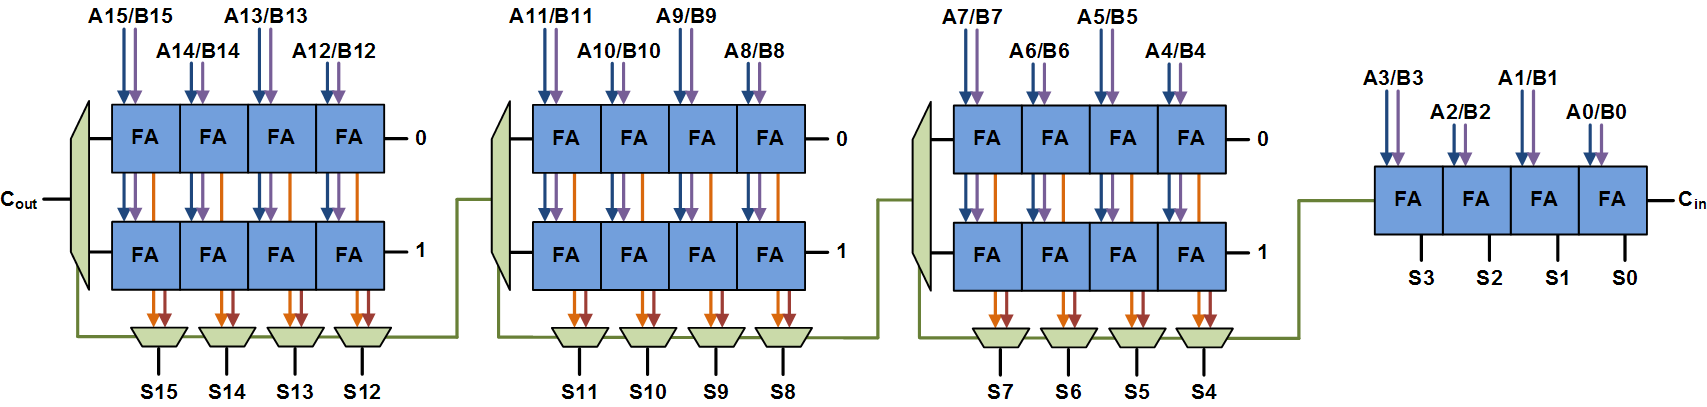
\includegraphics[width=2.5in]{select.png}
  \caption{Somador "ripple carry" 16bits com "carry select"}
  \label{fig:select}
\end{figure}

\section{Implementação}

Os alunos realizaram implmentação de um full adder de dois bits, bem como dos
MUX utilizados, afim de evitar o uso de estruturas da linguagem com 
implementação desconhecida.

Como a FPGA utilizada dispunha apenas de quatro displays "sete segmnetos", o
resultado foi exibido em hexadecimal (4 bits por display). Outra limitação da
placa foi a presença de apenas dez switches, portanto a entrada do usuário foi
dividida em quatro tempos; primeiro o usuário utiliza os oito primeiro switches
para informar o primeiro byte do primeiro operando, e pressiona o botão 0 para
confirmar a entrada. Posteriormente, utiliza os mesmos switches para o primeiro
byte do segundo operando, e aperta o botão 1, e assim por diante até todos
bytes de todos operandos serem entrados. Como existem apenas três botões, a
entrada do último byte do último operando é confirmada com a ativação do switch
9. O switch restante (switch 8) corresponde ao carry in.

\section{Conclusão}



\bibliographystyle{sbc}
\bibliography{main}

\end{document}
